

\documentclass[a4paper]{article}
\usepackage[a4paper,margin=1in]{geometry}
\usepackage{authblk}
\usepackage{booktabs}
\usepackage[shortlabels]{enumitem}
\usepackage[table,xcdraw]{xcolor}
\usepackage{graphicx}
\setlength\headheight{15pt}
\colorlet{headbgcolor}{orange}
\usepackage[markcase=noupper]{scrlayer-scrpage}
\usepackage[english]{babel}
\usepackage{hyperref}
\usepackage{adjustbox}
\usepackage{float}
\usepackage{blindtext}
\usepackage{multirow}
\usepackage{dcolumn}% Align table columns on decimal point
\usepackage{bm}% bold math
\usepackage{hyperref}% add hypertext capabilities
\usepackage[english]{babel}
\usepackage{caption}
\usepackage{subcaption}
\usepackage{siunitx}
\usepackage{amsmath}
\usepackage{tabularx}
\usepackage[super]{nth}
\clearpairofpagestyles
%\automark[chapter]{chapter}
%\renewcommand\chaptermarkformat{\chaptername\ \thechapter:\enskip}
\setlength{\parskip}{1em}
\renewcommand{\baselinestretch}{1.2}
\providecommand{\tightlist}{%
\setlength{\itemsep}{0pt}\setlength{\parskip}{0pt}}


\title{\textbf{Title}}
\author{Author}
\date{Date}

\begin{document}

\maketitle

\hypertarget{objective}{%
\section{Objective}\label{objective}}

\begin{itemize}
\tightlist
\item
To record the alpha spectrum of \(Am-241\) radioactive source at
different pressures.
\item
And to record the energy loss of alpha particles as a function of
pressure,
\item
And hence to determine the range of alpha radiation in air.
\end{itemize}

\hypertarget{apparatus}{%
\section{Apparatus}\label{apparatus}}

\begin{itemize}
\tightlist
\item
Alpha spectroscopy chamber with vaccum pump • Scintillation Detector
\item
Discriminator-preamplifier
\item
MCA Box
\item
HF Cables
\item
CASSY Lab software
\end{itemize}

\hypertarget{theory}{%
\section{Theory}\label{theory}}

Normal amplifiers, when amplifying weak signals, also amplifies the
noise present in it. This noise incldes flicker noise at low frequencies
which can be picked up from other electronics nearby, or thermal noise,
which spans all frequencies and is of thermodynamic origin. Thsese noise
signals can be ignored if we know the frequency of the signal we are
looking for. This is what a lock-in amplifier does, extracting the
signal given a known carrier wave. \[
R=\int_{E_0}^0 \frac{dx}{dE}\cdot dE dx
\]

\[
R \propto E_0^{3/2}
\]

\[
x = \frac{c}{c_0}\cdot x_0
\]

\hypertarget{determining-small-resistance}{%
\subsection{Determining Small
Resistance}\label{determining-small-resistance}}

Measuring small resistances using conventional techniques can be tricky,
since oftentimes, the resistance of the circuit itself can be higher
than the resistance we are dealing with, which gives us a lot of noise.
This can be solved by using lock-in amplifiers.

Using an AC signal, at each frequency, we plot a graph between
\(V_{DC}\) and \(V_{AC}\), and get the slope.

Since \(dV_{AC}=RdI_{AC}\)m where R is the resistance of the primary
circuit, and \(dI_{AC}\) is the change in current through the low
resistance when the signal generator voltage is changed by \(dV_{AC}\).
Also, the voltage \(V_r\) changes by \(dV_r\) where \(dV_r=rdI_{AC}\).
Therefore, we have:

\[
\frac{dV_{DC}}{dV_{AC}}=\mu \frac{r}{R}
\]

\hypertarget{determining-mutual-inductance}{%
\subsection{Determining Mutual
Inductance}\label{determining-mutual-inductance}}

Changing magnetic fields induces electric fields. Therefore, when a coil
of wire is connected to an oscillating voltage, the changing magnetic
fields due to it can induce an emf in a coil placed neaby.

Hence, if the current supplied to the primary coil is , then the emf
induced in the secondary coil is obtained as:

\[
V=-M\frac{dI}{dt}= -2\pi Mft_0 sin(2\pi f t+\frac{\pi}{2})
\]

From above, it is evident that the induced current and the primary
current are \(90^o\) out of phase. Also, the induced current is directly
proportional to the amplitude \(I_0\) of the primary current, and it's
frequency \(f\).

\hypertarget{observations}{%
\section{Observations}\label{observations}}

\begin{table}[htb]
    \centering
    \begin{tabular}{@{}cccccc@{}}
        \toprule
        Temperature (in $^oC$) & $V_R$ & $V_C$ & Capacitance (in nF) &  &  \\
        \midrule
        21.3 & 3.92 & 1.95 & 0.62 &  &  \\
        50 & 3.95 & 1.95 & 0.63 &  &  \\
        55 & 3.95 & 1.94 & 0.65 &  &  \\
        60 & 3.96 & 1.93 & 0.64 &  &  \\
        65 & 3.97 & 1.91 & 0.67 &  &  \\
        70 & 3.98 & 1.89 & 0.68 &  &  \\
        75 & 4 & 1.85 & 0.71 &  &  \\
        80 & 4.03 & 1.85 & 0.73 &  &  \\
        85 & 4.06 & 1.82 & 0.78 &  &  \\
        90 & 4.10 & 1.75 & 0.82 &  &  \\
        91 & 0.12 & 1.67 & 0.86 &  &  \\
        93 & 4.15 & 1.63 & 0.9 &  &  \\
        95 & 4.12 & 1.57 & 0.93 &  &  \\
        97 & 4.13 & 1.57 & 0.97 &  &  \\
        99 & 4.15 & 1.57 & 1.01 &  &  \\
        100 & 4.19 & 1.57 & 1.03 &  &  \\
        101 & 4.25 & 1.58 & 1.04 &  &  \\
        102 & 4.24 & 1.59 & 1.05 &  &  \\
        103 & 4.24 & 1.6 & 1.06 &  &  \\
        104 & 4.20 & 1.61 & 1.07 &  &  \\
        105 & 4.33 & 1.62 & 1.08 &  &  \\
        106 & 4.25 & 1.6 & 1.1 &  &  \\
        107 & 4.24 & 1.56 & 1.11 &  &  \\
        108 & 4.25 & 1.54 & 1.11 &  &  \\
        109 & 4.26 & 1.54 & 1.1 &  &  \\
        110 & 4.32 & 1.59 & 1.08 &  &  \\
        111 & 4.33 & 1.61 & 1.07 &  &  \\
        112 & 4.37 & 1.62 & 1.06 &  &  \\
        113 & 4.33 & 1.62 & 1.04 &  &  \\
        114 & 4.28 & 1.6 & 1.01 &  &  \\
        115 & 4.20 & 1.58 & 0.98 &  &  \\
        116 & 4.18 & 1.57 & 0.96 &  &  \\
        115 & 4.21 & 1.59 & 0.99 &  &  \\
        114 & 4.20 & 1.6 & 1.01 &  &  \\
        113 & 4.21 & 1.61 & 1.03 &  &  \\
        112 & 4.25 & 1.62 & 1.05 &  &  \\
        111 & 4.23 & 1.63 & 1.07 &  &  \\
        110 & 4.29 & 1.62 & 1.09 &  &  \\
        109 & 4.26 & 11.62 & 1.1 &  &  \\
        108 & 4.24 & 1.58 & 1.11 &  &  \\
        107 & 4.25 & 1.58 & 1.11 &  &  \\
        106 & 4.25 & 1.54 & 1.11 &  &  \\
        105 & 4.21 & 1.37 & 1.12 &  &  \\
        103 & 4.26 & 1.58 & 1.09 &  &  \\
        102 & 4.21 & 1.59 & 1.08 &  &  \\
        101 & 4.25 & 1.6 & 1.07 &  &  \\
        100 & 4.2 & 1.57 & 1.05 &  &  \\
        99 & 4.15 & 1.56 & 1.03 &  &  \\
        97 & 4.2 & 1.54 & 1.00 &  &  \\
        95 & 4.17 & 1.54 & 0.95 &  &  \\
        93 & 4.15 & 1.51 & 0.92 &  &  \\
        91 & 4.07 & 1.5 & 0.88 &  &  \\
        90 & 4.07 & 1.49 & 0.86 &  &  \\
        85 & 4.04 & 1.45 & 0.8 &  &  \\
        75 & 3.58 & 1.43 & 0.73 &  &  \\
        70 & 3.96 & 2.12 & 0.7 &  &  \\
        graph(0;3) &  &  &  &  &  \\
        \bottomrule
    \end{tabular}
\end{table}

\hypertarget{graphs}{%
\section{Graphs}\label{graphs}}

\begin{center} 
\begin{figure}[H] 
\begin{center}
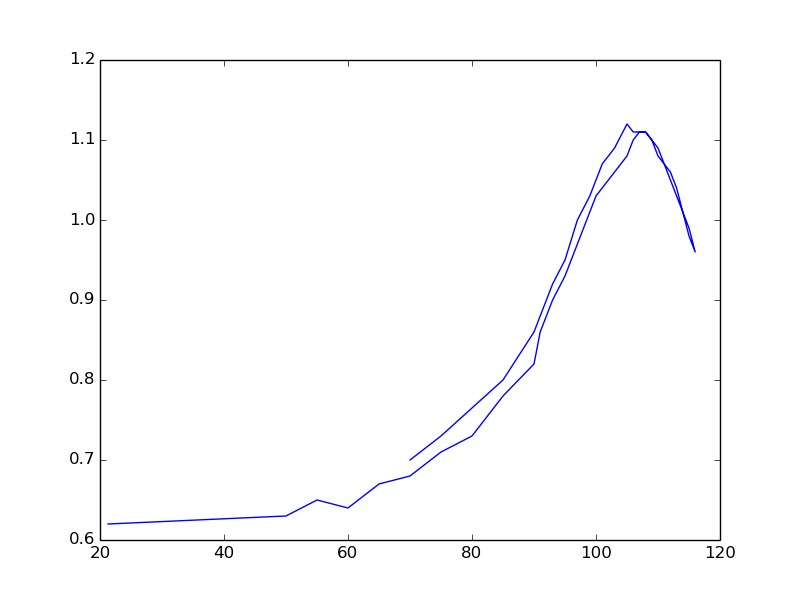
\includegraphics[scale = 0.5]{graphs/03table1.png}
\caption{Normal Transverse Zeeman Effect} 
\end{center}
\end{figure}
\end{center}

\hypertarget{results}{%
\section{Results}\label{results}}

\begin{itemize}
\tightlist
\item
The amplification factor was obtained as: \(\mu = 1.805 \times 10^3\)
\item
The small resistance was obtained to be: \(r =0.031\Omega\)
\item
The mutual inductance of the given coil was obtained as:
\(M = 120.20 \mu H\)
\end{itemize}

\hypertarget{conclusion}{%
\section{Conclusion}\label{conclusion}}

The functioning of a lock-in amplifier, and its use in extracting signal
from noise using phase modulation of the reference signal was studied.
These were used in obtaining the resistance of a given small resistance,
and the mutual inductance of a given coil.
\end{document}
